\mfpicnumber{1}

\opengraphsfile{Polydivision}

\setcounter{footnote}{0}

\label{Polydivision}


Suppose we wish to find the zeros of $f(x) = x^3 + 4x^2-5x-14$.  Setting $f(x)=0$ results in the polynomial equation $x^3 + 4x^2-5x-14=0$.   Despite all of the factoring techniques we learned\footnote{and probably forgot} in Intermediate Algebra, this equation foils\footnote{pun intended} us at every turn.  If we graph $f$ using the graphing calculator, we get

\smallskip

\centerline{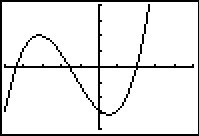
\includegraphics[width=2in]{./PolynomialsGraphics/PolyDiv01.jpg}}

\smallskip

The graph suggests that the function has three zeros, one of which is $x=2$.  It's easy to show that $f(2) = 0$, but the other two zeros seem to be less friendly.  Even though we could use the `Zero' command to find decimal approximations for these, we seek a method to find the remaining zeros \emph{exactly}.  Based on our experience, if $x=2$ is a zero, it seems that there should be a factor of $(x-2)$ lurking around in the factorization of $f(x)$.  In other words, we should expect that $x^3 + 4x^2-5x-14=(x-2) \, q(x)$, where $q(x)$ is some other polynomial.  How could we find such a $q(x)$, if it even exists?  The answer comes from our old friend, polynomial division. Dividing $x^3 + 4x^2-5x-14$ by $x-2$ gives

\setlength\arraycolsep{0.1pt}
\setlength\extrarowheight{2pt}

\[ \begin{array}{cccccccccc}

& & & & & x^2 & + & 6x & + & 7 \\ \hhline{~~~|-------}

x & - & 2 \, \vline& x^3 & + & 4x^2 & - & 5x & - & 14 \\

 &  &  -& \left(x^3 \right. & - & \left.  2x^2\right) &  &  &  &  \\ \hhline{~~~---~~~~} 
 &  &  &   &  & 6 x^2 & - & 5x &  &  \\ 
 &  &  &   & - & \left(6 x^2 \right. & - & \left. 12x \right) &  &  \\ \hhline{~~~~~---~~} 
 &  &  &   &   &  & & 7x  & - & 14 \\
 &  &  &   &   &  & - & \left( 7x \right. & - & \left. 14 \right) \\ \hhline{~~~~~~~---} 
 &   &  &  &  &  &  &  &  & 0
 
\end{array}\]

\setlength\arraycolsep{5pt}
\setlength\extrarowheight{0pt}

As you may recall, this means $x^3 + 4x^2-5x-14=(x-2)\left(x^2+6x+7\right)$, so to find the zeros of $f$, we now solve $(x-2)\left(x^2+6x+7\right)=0$.   We get $x-2=0$ (which gives us our known zero, $x=2$) as well as $x^2+6x+7=0$.   The latter doesn't factor nicely, so we apply the Quadratic Formula to get $x = -3 \pm \sqrt{2}$.  The point of this section is to generalize the technique applied here.  First up is a friendly reminder of what we can expect when we divide polynomials.

\smallskip

\colorbox{ResultColor}{\bbm

\begin{thm} \label{polydiv} \textbf{Polynomial Division:}  Suppose $d(x)$ and $p(x)$ are nonzero polynomials where the degree of $p$ is greater than or equal to the degree of $d$.  There exist two unique polynomials, $q(x)$ and $r(x)$, such that $p(x) = d(x) \, q(x) + r(x),\,$ where either $r(x) = 0$ or the degree of $r$ is strictly less than the degree of $d$.
\end{thm}
\ebm}

\smallskip

As you may recall, all of the polynomials in Theorem \ref{polydiv} have special names.  The polynomial $p$ is called the \index{polynomial division ! dividend} \textbf{dividend}; $d$ is the \index{polynomial division ! divisor} \textbf{divisor}; $q$ is the \index{polynomial division ! quotient} \textbf{quotient}; $r$ is the \index{polynomial division ! remainder} \textbf{remainder}.  If $r(x)=0$ then $d$ is called a \index{polynomial division ! factor} \textbf{factor} of $p$.  The proof of Theorem \ref{polydiv} is usually relegated to a course in Abstract Algebra,\footnote{Yes, Virginia, there are Algebra courses more abstract than this one.} but we can still use the result to establish two important facts which are the basis of the rest of the chapter.

\smallskip

\colorbox{ResultColor}{\bbm

\begin{thm} \label{remainderthm}\index{Remainder Theorem}\textbf{The Remainder Theorem:}  Suppose $p$ is a polynomial of degree at least $1$ and $c$ is a real number.  When $p(x)$ is divided by $x-c$ the remainder is $p(c)$.  

\end{thm}
\ebm}

\smallskip


The proof of Theorem \ref{remainderthm} is a direct consequence of Theorem \ref{polydiv}.  When a polynomial is divided by $x-c$, the remainder is either $0$ or has degree less than the degree of $x-c$.  Since $x-c$ is degree $1$, the degree of the remainder must be $0$, which means the remainder is a constant.  Hence, in either case, $p(x) = (x-c) \, q(x) + r$, where $r$, the remainder, is a real number, possibly $0$.  It follows that $p(c) = (c-c) \, q(c) + r = 0 \cdot q(c) + r = r$, so we get $r = p(c)$ as required.  There is one last `low hanging fruit'\footnote{Jeff hates this expression and Carl included it just to annoy him.} to collect which we present below.

\smallskip

\colorbox{ResultColor}{\bbm

\begin{thm} \label{factorthm}\index{Factor Theorem}\textbf{The Factor Theorem:}  Suppose $p$ is a nonzero polynomial.  The real number $c$ is a zero of $p$ if and only if $(x-c)$ is a factor of $p(x)$.  

\end{thm}
\ebm}

\smallskip

The proof of The Factor Theorem is a consequence of what we already know.  If $(x-c)$ is a factor of $p(x)$, this means $p(x) = (x-c) \, q(x)$ for some polynomial $q$.  Hence, $p(c) = (c-c) \, q(c) = 0$, so $c$ is a zero of $p$.  Conversely, if $c$ is a zero of $p$, then $p(c) = 0$. In this case, The Remainder Theorem tells us the remainder when $p(x)$ is divided by $(x-c)$, namely $p(c)$, is $0$, which means $(x-c)$ is a factor of $p$.  What we have established is the fundamental connection between zeros of polynomials and factors of polynomials.  

\smallskip

Of the things The Factor Theorem tells us, the most pragmatic is that we had better find a more efficient way to divide polynomials by quantities of the form $x-c$.  Fortunately, people like \href{http://en.wikipedia.org/wiki/Synthetic_division}{\underline{Ruffini}} and \href{http://en.wikipedia.org/wiki/Horner_scheme}{\underline{Horner}} have already blazed this trail.  Let's take a closer look at the long division we performed at the beginning of the section and try to streamline it.  First off, let's change all of the subtractions into additions by distributing through the $-1$s.


\setlength\arraycolsep{0.1pt}
\setlength\extrarowheight{2pt}

\[ \begin{array}{cccccccccc}

& & & & & x^2 & + & 6x & + & 7 \\ \hhline{~~~|-------}

x & - & 2 \, \vline& x^3 & + & 4x^2 & - & 5x & - & 14 \\

 &  &  &  -x^3  & + &   2x^2 &  &  &  &  \\ \hhline{~~~---~~~~} 
 &  &  &   &  & 6 x^2 & - & 5x &  &  \\ 
 &  &  &   & &-6 x^2  & + &  12x &  &  \\ \hhline{~~~~~---~~} 
 &  &  &   &   &  & & 7x  & - & 14 \\
 &  &  &   &   &  & & - 7x  & + &  14  \\ \hhline{~~~~~~~---} 
 &   &  &  &  &  &  &  &  & 0
 
\end{array}\]

\setlength\arraycolsep{5pt}
\setlength\extrarowheight{0pt}


Next, observe that the terms $-x^3$, $-6x^2$ and $-7x$ are the exact opposite of the terms above them.  The algorithm we use ensures this is always the case, so we can omit them without losing any information. Also note that the terms we `bring down' (namely the $-5x$ and $-14$) aren't really necessary to recopy, so we omit them, too.


\setlength\arraycolsep{0.1pt}
\setlength\extrarowheight{2pt}

\[ \begin{array}{cccccccccc}

& & & & & x^2 & + & 6x & + & 7 \\ \hhline{~~~|-------}

x & - & 2 \, \vline& \, \, x^3 & + & 4x^2 & - & 5x & - & 14 \\

 &  &  &   &  &   2x^2 &  &  &  &  \\ \hhline{~~~---~~~~} 
 &  &  &   &  & 6 x^2 &  &  &  &  \\ 
 &  &  &   & &  &  &  12x &  &  \\ \hhline{~~~~~---~~} 
 &  &  &   &   &  & & 7x  &  &  \\
 &  &  &   &   &  & &   &  &  14  \\ \hhline{~~~~~~~---} 
 &   &  &  &  &  &  &  &  & 0
 
\end{array}\]

\setlength\arraycolsep{5pt}
\setlength\extrarowheight{0pt}

Now, let's move things up a bit and, for reasons which will become clear in a moment, copy the $x^3$ into the last row.


\setlength\arraycolsep{0.1pt}
\setlength\extrarowheight{2pt}

\[ \begin{array}{cccccccccc}

& & & & & x^2 & + & 6x & + & 7 \\ \hhline{~~~|-------}

x & - & 2 \, \vline& \, \, x^3 & + & 4x^2 & - & 5x & - & 14 \\

 &  &  &   & &   2x^2 &  & 12x &  & 14 \\ \hhline{~~~-------} 
 &  &  & x^3  &  & 6 x^2 &  & 7x &  &0  \\  
\end{array}\]

\setlength\arraycolsep{5pt}
\setlength\extrarowheight{0pt}

Note that by arranging things in this manner, each term in the last row is obtained by adding the two terms above it.  Notice also that the quotient polynomial can be obtained by dividing each of the first three terms in the last row by $x$ and adding the results.   If you take the time to work back through the original division problem, you will find that this is exactly the way we determined the quotient polynomial.  This means that we no longer need to write the quotient polynomial down, nor the $x$ in the divisor, to determine our answer.

\setlength\arraycolsep{0.1pt}
\setlength\extrarowheight{2pt}

\[ \begin{array}{cccccccccc}


 & & - 2 \, \, \vline& \, \, x^3 & + & 4x^2 & - & 5x & - & 14 \\

 &  &  &   & &   2x^2 &  & 12x &  & 14 \\ \hhline{~~~-------} 
 &  &  & x^3  &  & 6 x^2 &  & 7x &  &0  \\  
\end{array}\]

\setlength\arraycolsep{5pt}
\setlength\extrarowheight{0pt}

We've streamlined things quite a bit so far, but we can still do more.  Let's take a moment to remind ourselves where the $2x^2$, $12x$ and $14$ came from in the second row.  Each of these terms was obtained by multiplying the terms in the quotient, $x^2$, $6x$ and $7$, respectively, by the $-2$ in $x-2$,  then by $-1$ when we changed the subtraction to addition.  Multiplying by $-2$ then by $-1$ is the same as multiplying by $2$, so we replace the $-2$ in the divisor by $2$.   Furthermore, the coefficients of the quotient polynomial match the coefficients of the first three terms in the last row, so we now take the plunge and write only the coefficients of the terms to get



\[ \begin{array}{rrrrr}


  2 \, \, \vline& 1 & 4 & -5  & -14 \\

   &&   2 &   12 &   14 \\ \hhline{~----} 
  & 1  &   6  &  7 &  0  \\  
\end{array}\]



We have constructed a \index{polynomial division ! synthetic division}\index{synthetic division tableau}\textbf{synthetic division tableau} for this polynomial division problem.  Let's re-work our division problem using this tableau to see how it greatly streamlines the division process.  To divide $x^3+4x^2-5x-14$ by $x-2$, we write $2$ in the place of the divisor and the coefficients of $x^3+4x^2-5x-14$ in for the dividend.  Then `bring down' the first coefficient of the dividend.

\bigskip

\begin{center}

\begin{tabular}{cc}

$ \begin{array}{rrrrr}


  2 \, \, \vline& 1 & 4 & -5  & -14 \\

   &  &    &    &  \\ \hhline{~----} 
  &   &     &   &    \\  
\end{array}$  \hspace{1in}
&


$ \begin{array}{rrrrr}


  2 \, \, \vline& 1 & 4 & -5  & -14 \\

   & \downarrow &    &    &  \\ \hhline{~----} 
  & 1  &     &   &    \\  
\end{array}$ \\

\end{tabular}

\end{center}

\bigskip

Next, take the $2$ from the divisor and multiply by the $1$ that was `brought down' to get $2$.  Write this underneath the $4$, then add to get $6$.

\bigskip

\begin{center}

\begin{tabular}{cc}

$ \begin{array}{rrrrr}


  2 \, \, \vline& 1 & 4 & -5  & -14 \\

   & \downarrow  &  2  &    &  \\ \hhline{~----} 
  & 1  &     &   &    \\  
\end{array}$ \hspace{1in}
&


$ \begin{array}{rrrrr}


  2 \, \, \vline& 1 & 4 & -5  & -14 \\

   & \downarrow &  2  &    &  \\ \hhline{~----} 
  & 1  &   6  &   &    \\  
\end{array}$ \\


\end{tabular}

\end{center}

\bigskip

Now take the $2$ from the divisor times the $6$ to get $12$, and add it to the $-5$ to get $7$.

\bigskip

\begin{center}

\begin{tabular}{cc}


$ \begin{array}{rrrrr}


  2 \, \, \vline& 1 & 4 & -5  & -14 \\

   & \downarrow &  2  &  12  &  \\ \hhline{~----} 
  & 1  &   6  &   &    \\  
\end{array}$ \hspace{1in}

&

$ \begin{array}{rrrrr}


  2 \, \, \vline& 1 & 4 & -5  & -14 \\

   & \downarrow &  2  &  12  &  \\ \hhline{~----} 
  & 1  &   6  & 7  &    \\  
\end{array}$ \\


\end{tabular}

\end{center}


Finally, take the $2$ in the divisor times the $7$ to get $14$, and add it to the $-14$ to get $0$.

\bigskip

\begin{center}

\begin{tabular}{cc}

$ \begin{array}{rrrrr}


  2 \, \, \vline& 1 & 4 & -5  & -14 \\

   & \downarrow &  2  &  12  & 14 \\ \hhline{~----} 
  & 1  &   6  & 7  &    \\  
\end{array}$ \hspace{1in} 

&

$ \begin{array}{rrrrr}


  2 \, \, \vline& 1 & 4 & -5  & -14 \\

   & \downarrow &  2  &  12  & 14 \\ \hhline{~----} 
  & 1  &   6  & 7  &  \fbox{$0$}  \\  
\end{array}$ \\



\end{tabular}

\end{center}

The first three numbers in the last row of our tableau are the coefficients of the quotient polynomial.  Remember, we started with a third degree polynomial and divided by a first degree polynomial, so the quotient is a second degree polynomial.  Hence the quotient is $x^2+6x+7$.  The number in the box is the remainder.  Synthetic division is our tool of choice for dividing polynomials by divisors of the form $x-c$.  It is important to note that it works \emph{only} for these kinds of divisors.\footnote{You'll need to use good old-fashioned polynomial long division for divisors of degree larger than 1.} Also take note that when a polynomial (of degree at least $1$) is divided by $x-c$, the result will be a polynomial of exactly one less degree. Finally, it is  worth the time to trace each step in synthetic division back to its corresponding step in long division.  While the authors have done their best to indicate where the algorithm comes from, there is no substitute for working through it yourself.

\begin{ex}  Use synthetic division to perform the following polynomial divisions.  Find the quotient and the remainder polynomials, then write the dividend, quotient and remainder in the form given in Theorem \ref{polydiv}.

\begin{multicols}{3}
\begin{enumerate}

\item  $\left(5x^3 - 2x^2 + 1\right) \div (x-3)$ \vphantom{$\dfrac{4-8x-12x^2}{2x-3}$}
\item  $\left(x^3+8\right) \div (x+2)$ \vphantom{$\dfrac{4-8x-12x^2}{2x-3}$}
\item  $\dfrac{4-8x-12x^2}{2x-3}$

\end{enumerate}
\end{multicols}

{ \bf Solution.} 

\begin{enumerate}


\item When setting up the synthetic division tableau, we need to enter $0$ for the coefficient of $x$ in the dividend.  Doing so gives


\[ \begin{array}{rrrrr}


  3 \, \, \vline& 5 & -2 & 0  & 1 \\

   & \downarrow &  15  &  39  & 117 \\ \hhline{~----} 
  & 5  &   13  & 39  &  \fbox{$118$}  \\  
\end{array}\]

Since the dividend was a third degree polynomial, the quotient is a quadratic polynomial with coefficients $5$, $13$ and $39$.  Our quotient is $q(x) = 5x^2+13x+39$ and the remainder is $r(x) = 118$.  According to Theorem \ref{polydiv}, we have $5x^3 - 2x^2 + 1 = (x-3)\left(5x^2+13x+39 \right) + 118$.

\item  For this division, we rewrite $x+2$ as $x-(-2)$ and proceed as before

\[ \begin{array}{rrrrr}


  -2 \, \, \vline& 1 & 0 & 0  & 8 \\

   & \downarrow &  -2  &  4  & -8 \\ \hhline{~----} 
  & 1  &   -2  & 4  &  \fbox{$0$}  \\  
\end{array}\]

We get the quotient $q(x) = x^2-2x+4$ and the remainder $r(x) =0$. Relating the dividend, quotient and remainder gives $x^3+8 = (x+2)\left( x^2-2x+4 \right)$.  

\item To divide $4-8x-12x^2$ by $2x-3$, two things must be done.  First, we write the dividend in descending powers of $x$ as $-12x^2-8x+4$.  Second, since synthetic division works only for factors of the form $x-c$, we factor $2x-3$ as $2\left(x-\frac{3}{2}\right)$.  Our strategy is to first divide $-12x^2-8x+4$ by $2$, to get $-6x^2-4x+2$.  Next, we divide by $\left(x-\frac{3}{2}\right)$.  The tableau becomes

\[ \begin{array}{rrrr}


  \frac{3}{2} \, \, \vline& -6 & -4 & 2   \\ [4pt]

   & \downarrow &  -9  & -\frac{39}{2}  \\ [4pt] \hhline{~---} 
  &  -6  &   -13  & \fbox{$-\frac{35}{2}$}  \\  
\end{array}\]


\end{enumerate}

From this, we get $-6x^2-4x+2 = \left(x-\frac{3}{2}\right)(-6 x - 13) - \frac{35}{2}$.  Multiplying both sides by $2$ and distributing gives $-12x^2-8x+4 = \left(2x-3\right) (-6 x - 13) - 35$.  At this stage, we have written $-12x^2-8x+4$ in the \textbf{form} $(2x-3) q(x) + r(x)$, but how can we be sure the quotient polynomial is $-6x-13$ and the remainder is $-35$?  The answer is the word `unique' in Theorem \ref{polydiv}.  The theorem states that there is only one way to decompose $-12x^2-8x+4$ into a multiple of $(2x-3)$  plus a constant term.  Since we have found such a way, we can be sure it is the only way. \qed


\end{ex}

The next example pulls together all of the concepts discussed in this section.  

\begin{ex} Let $p(x) = 2x^3-5x+3$.

\begin{enumerate}

\item  Find $p(-2)$ using The Remainder Theorem.  Check your answer by substitution.

\item  Use the fact that $x=1$ is a zero of $p$ to factor $p(x)$ and then find all of the real zeros of $p$.

\end{enumerate}

{\bf Solution.}

\begin{enumerate}

\item  The Remainder Theorem states $p(-2)$ is the remainder when $p(x)$ is divided by $x-(-2)$.  We set up our synthetic division tableau below.  We are careful to record the coefficient of $x^2$ as $0$, and proceed as above.

\[\begin{array}{rrrrr}
 -2 \, \, \vline& 2 & 0 & -5  & 3 \\

   & \downarrow &  -4  &  8  & -6 \\ \hhline{~----} 
  & 2  &   -4  & 3 &  \fbox{$-3$}  \\  
\end{array}\]

According to the Remainder Theorem, $p(-2) = -3$.  We can check this by direct substitution into the formula for $p(x)$:  $p(-2) = 2(-2)^3-5(-2)+3 = -16+10+3=-3$.

\item The Factor Theorem tells us that since $x=1$ is a zero of $p$, $x-1$ is a factor of $p(x)$.  To factor $p(x)$, we divide

\[\begin{array}{rrrrr}
 1 \, \, \vline& 2 & 0 & -5  & 3 \\

   & \downarrow &  2  &  2  & -3 \\ \hhline{~----} 
  & 2  &   2  & -3 &  \fbox{$0$}  \\  
\end{array}\]

We get a remainder of $0$ which verifies that, indeed, $p(1) = 0$.  Our quotient polynomial is a second degree polynomial with coefficients $2$, $2$, and $-3$. So $q(x) = 2x^2 + 2x - 3$.  Theorem \ref{polydiv} tells us $p(x) = (x-1)\left( 2x^2 + 2x - 3\right)$.  To find the remaining real zeros of $p$, we need to solve $2x^2 + 2x - 3=0$ for $x$.  Since this doesn't factor nicely, we use the quadratic formula to find that the remaining zeros are $x = \frac{-1 \pm \sqrt{7}}{2}$. \qed
\end{enumerate}
\end{ex}

In Section \ref{GraphsofPolynomials}, we discussed the notion of the multiplicity of a zero.  Roughly speaking, a zero with multiplicity $2$ can be divided twice into a polynomial;  multiplicity $3$, three times and so on.  This is illustrated in the next example.

\begin{ex}  Let $p(x) = 4x^4-4x^3-11x^2+12x-3$.  Given that $x=\frac{1}{2}$ is a zero of multiplicity $2$,  find all of the real zeros of $p$.

\smallskip

{\bf Solution.}  We set up for synthetic division.  Since we are told the multiplicity of $\frac{1}{2}$ is two, we continue our tableau and divide $\frac{1}{2}$ into the quotient polynomial

\[\begin{array}{rrrrrr}
 \frac{1}{2} \, \, \vline& 4 & -4 & -11  & 12 & -3 \\

   & \downarrow &  2  &  -1  & -6 & 3\\ \hhline{~-----} 
   
  \frac{1}{2} \, \, \vline&  4  &   -2  & -12 & 6 &  \fbox{$0$}  \\
    
      & \downarrow &  2  &  0  & -6 &\\ \hhline{~----} 
      
       & 4  &   0  & -12 & \fbox{0} &   \\  



\end{array}\]

From the first division, we get $4x^4-4x^3-11x^2+12x-3=\left(x-\frac{1}{2}\right) \left(4x^3-2x^2-12x+6\right)$.  The second division tells us $4x^3-2x^2-12x+6=\left(x-\frac{1}{2}\right)\left(4x^2-12\right)$.  Combining these results, we have  $4x^4-4x^3-11x^2+12x-3 = \left(x-\frac{1}{2}\right)^2\left(4x^2-12\right)$.  To find the remaining zeros of $p$, we set $4x^2-12=0$ and get $x = \pm \sqrt{3}$.  \qed

\end{ex}

A couple of things about the last example are worth mentioning. First, the extension of the synthetic division tableau for repeated divisions will be a common site in the sections to come. Typically, we will start with a higher order polynomial and peel off one zero at a time until we are left with a quadratic, whose roots can always be found using the Quadratic Formula.  Secondly, we found $x = \pm \sqrt{3}$ are zeros of $p$.  The Factor Theorem guarantees $\left(x-\sqrt{3}\right)$ and $\left(x - \left(-\sqrt{3}\right)\right)$ are both factors of $p$.  We can certainly put the Factor Theorem to the test and continue the synthetic division tableau from above to see what happens.

\[\begin{array}{rrrrrr}
 \frac{1}{2} \, \, \vline& 4 & -4 & -11  & 12 & -3 \\

  & \downarrow &  2  &  -1  & -6 & 3\\ \hhline{~-----} 
  
  \frac{1}{2} \, \, \vline&  4  &   -2  & -12 & 6 &  \fbox{$0$}  \\
    
  & \downarrow &  2  &  0  & -6 &\\ \hhline{~----} 
 
  
 \sqrt{3} \, \, \vline  & 4  &   0  & -12 & \fbox{0} &   \\
  
                        & \downarrow &  4\sqrt{3}  & 12  & &\\ \hhline{~---} 
 
   -\sqrt{3} \, \, \vline  & 4  &  4\sqrt{3}  & \fbox{0} &  &   \\  
       
                          & \downarrow &  -4\sqrt{3}  &   & &\\ \hhline{~--} 
       
													& 4  &  \fbox{0}  &  &  &   \\

\end{array}\]

This gives us $4x^4-4x^3-11x^2+12x-3=\left(x-\frac{1}{2}\right)^2 \left(x-\sqrt{3}\right)\left(x - \left(-\sqrt{3}\right)\right) (4)$, or, when written with the constant in front \[ p(x) = 4\left(x-\frac{1}{2}\right)^2 \left(x-\sqrt{3}\right)\left(x - \left(-\sqrt{3}\right)\right)\]

We have shown that $p$ is a product of its leading coefficient times linear factors of the form $(x-c)$ where $c$ are zeros of $p$. It may surprise and delight the reader that, in theory, all polynomials can be reduced to this kind of factorization.  We leave that discussion to Section \ref{ComplexZeros}, because the zeros may not be real numbers.  Our final theorem in the section gives us an upper bound on the number of real zeros. 

\medskip

\colorbox{ResultColor}{\bbm
\begin{thm}  \label{nzerosreal} Suppose $f$ is a polynomial of degree $n \geq 1$.  Then $f$ has at most $n$ real zeros, counting multiplicities.

\end{thm}
\ebm}

\medskip

Theorem \ref{nzerosreal} is a consequence of the Factor Theorem and polynomial multiplication.  Every zero $c$ of $f$ gives us a factor of the form $(x-c)$ for $f(x)$.  Since $f$ has degree $n$, there can be at most $n$ of these factors.  The next section provides us some tools which not only help us determine where the real zeros are to be found, but which real numbers they may be.

\medskip

We close this section with a summary of several concepts previously presented.  You should take the time to look back through the text to see where each concept was first introduced and where each connection to the other concepts was made.

\medskip

\colorbox{ResultColor}{\bbm

\centerline{\textbf{Connections Between Zeros, Factors and Graphs of Polynomial Functions}}

\medskip

\hspace{.17in} Suppose $p$ is a polynomial function of degree $n \geq 1$.  The following statements are equivalent:

\begin{itemize}

\item The real number $c$ is a zero of $p$
\item $p(c) = 0$
\item $x = c$ is a solution to the polynomial equation $p(x) = 0$
\item $(x - c)$ is a factor of $p(x)$
\item The point $(c, 0)$ is an $x$-intercept of the graph of $y = p(x)$

\end{itemize}

\ebm}

\newpage

\subsection{Exercises}

In Exercises \ref{polydivreviewfirst} - \ref{polydivreviewlast}, use polynomial long division to perform the indicated division.  Write the polynomial in the form $p(x) = d(x)q(x) + r(x)$.

\begin{multicols}{2}
\begin{enumerate}

\item $\left(4x^2+3x-1 \right) \div (x-3)$ \label{polydivreviewfirst}
\item $\left(2x^3-x+1 \right) \div \left(x^{2} +x+1 \right)$ 

\setcounter{HW}{\value{enumi}}
\end{enumerate}
\end{multicols}

\begin{multicols}{2}
\begin{enumerate}
\setcounter{enumi}{\value{HW}}

\item $\left(5x^{4} - 3x^{3} + 2x^{2} - 1 \right) \div \left(x^{2} + 4 \right)$
\item $\left(-x^{5} + 7x^{3} - x \right) \div \left(x^{3} - x^{2} + 1 \right)$

\setcounter{HW}{\value{enumi}}
\end{enumerate}
\end{multicols}

\begin{multicols}{2}
\begin{enumerate}
\setcounter{enumi}{\value{HW}}

\item $\left(9x^{3} + 5 \right) \div \left(2x - 3 \right)$
\item $\left(4x^2 - x - 23 \right) \div \left(x^{2} - 1 \right)$ \label{polydivreviewlast}

\setcounter{HW}{\value{enumi}}
\end{enumerate}
\end{multicols}

In Exercises \ref{synthdivreviewfirst} - \ref{synthdivreviewlast} use synthetic division to perform the indicated division.  Write the polynomial in the form $p(x) = d(x)q(x) + r(x)$.

\begin{multicols}{2}
\begin{enumerate}
\setcounter{enumi}{\value{HW}}

\item $\left(3x^2-2x+1 \right) \div \left(x-1\right)$ \label{synthdivreviewfirst}
\item $\left(x^2-5 \right) \div \left(x-5\right)$

\setcounter{HW}{\value{enumi}}
\end{enumerate}
\end{multicols}

\begin{multicols}{2}
\begin{enumerate}
\setcounter{enumi}{\value{HW}}

\item $\left(3-4x-2x^2 \right) \div \left(x+1\right)$
\item $\left(4x^2-5x +3\right) \div \left(x+3\right)$

\setcounter{HW}{\value{enumi}}
\end{enumerate}
\end{multicols}

\begin{multicols}{2}
\begin{enumerate}
\setcounter{enumi}{\value{HW}}

\item $\left(x^3 + 8 \right) \div \left(x+2\right)$
\item $\left(4x^3 +2x-3 \right) \div \left(x -3\right)$

\setcounter{HW}{\value{enumi}}
\end{enumerate}
\end{multicols}

\begin{multicols}{2}
\begin{enumerate}
\setcounter{enumi}{\value{HW}}

\item $\left(18x^2-15x-25\right) \div \left(x - \frac{5}{3} \right)$
\item $\left(4x^2-1 \right) \div \left(x - \frac{1}{2} \right)$

\setcounter{HW}{\value{enumi}}
\end{enumerate}
\end{multicols}

\begin{multicols}{2}
\begin{enumerate}
\setcounter{enumi}{\value{HW}}

\item $\left(2x^3+x^2+2x+1 \right) \div \left(x + \frac{1}{2} \right)$
\item $\left(3x^3 - x + 4 \right) \div \left(x - \frac{2}{3} \right)$

\setcounter{HW}{\value{enumi}}
\end{enumerate}
\end{multicols}

\begin{multicols}{2}
\begin{enumerate}
\setcounter{enumi}{\value{HW}}

\item $\left(2x^3 - 3x +1 \right) \div \left(x - \frac{1}{2} \right)$
\item $\left(4x^4-12x^3+13x^2 -12x+9\right) \div \left(x - \frac{3}{2} \right)$

\setcounter{HW}{\value{enumi}}
\end{enumerate}
\end{multicols}

\begin{multicols}{2}
\begin{enumerate}
\setcounter{enumi}{\value{HW}}

\item $\left(x^4-6x^2+9 \right) \div \left(x -\sqrt{3} \right)$
\item $\left(x^6-6x^4+12x^2-8\right) \div \left(x +\sqrt{2} \right)$ \label{synthdivreviewlast}

\setcounter{HW}{\value{enumi}}
\end{enumerate}
\end{multicols}

In Exercises \ref{remainderexerfirst} - \ref{remainderexerlast}, determine $p(c)$ using the Remainder Theorem for the given polynomial functions and value of $c$.  If $p(c) = 0$, factor $p(x) = (x-c) q(x)$.

\begin{multicols}{2}
\begin{enumerate}
\setcounter{enumi}{\value{HW}}

\item $p(x) = 2x^2 - x + 1$, $c = 4$ \label{remainderexerfirst}
\item $p(x) = 4x^2-33x-180$, $c = 12$

\setcounter{HW}{\value{enumi}}
\end{enumerate}
\end{multicols}


\begin{multicols}{2}
\begin{enumerate}
\setcounter{enumi}{\value{HW}}

\item $p(x) = 2x^3 - x + 6$, $c=-3$
\item $p(x) = x^3+2x^2+3x+4$, $c =-1$

\setcounter{HW}{\value{enumi}}
\end{enumerate}
\end{multicols}

\begin{multicols}{2}
\begin{enumerate}
\setcounter{enumi}{\value{HW}}

\item $p(x) =3x^3-6x^2+4x-8$, $c=2$
\item $p(x) = 8x^3+12x^2+6x+1$, $c =-\frac{1}{2}$

\setcounter{HW}{\value{enumi}}
\end{enumerate}
\end{multicols}

\begin{multicols}{2}
\begin{enumerate}
\setcounter{enumi}{\value{HW}}

\item $p(x) = x^4 - 2x^2+4$, $c=\frac{3}{2}$
\item $p(x) = 6x^4-x^2+2$, $c =-\frac{2}{3}$

\setcounter{HW}{\value{enumi}}
\end{enumerate}
\end{multicols}


\begin{multicols}{2}
\begin{enumerate}
\setcounter{enumi}{\value{HW}}

\item $p(x) = x^4 +x^3-6x^2-7x-7$, $c=-\sqrt{7}$
\item $p(x) = x^2-4x+1$, $c =2-\sqrt{3}$ \label{remainderexerlast}

\setcounter{HW}{\value{enumi}}
\end{enumerate}
\end{multicols}

\newpage

In Exercises \ref{factorpolyzerofirst} - \ref{factorpolyzerolast}, you are given a polynomial and one of its zeros.  Use the techniques in this section to find the rest of the real zeros and factor the polynomial.  

\begin{multicols}{2}
\begin{enumerate}
\setcounter{enumi}{\value{HW}}

\item $x^{3} - 6x^{2} + 11x - 6, \;\; c = 1$ \label{factorpolyzerofirst}
\item $x^{3} - 24x^{2} + 192x - 512, \;\; c = 8$

\setcounter{HW}{\value{enumi}}
\end{enumerate}
\end{multicols}

\begin{multicols}{2}
\begin{enumerate}
\setcounter{enumi}{\value{HW}}

\item $3x^{3} + 4x^{2} - x - 2, \;\; c = \frac{2}{3}$
\item $2x^3-3x^2-11x+6, \;\; c=\frac{1}{2}$

\setcounter{HW}{\value{enumi}}
\end{enumerate}
\end{multicols}

\begin{multicols}{2}
\begin{enumerate}
\setcounter{enumi}{\value{HW}}

\item $x^3+2x^2-3x-6, \;\; c = -2$
\item $2x^3-x^2-10x+5, \;\; c=\frac{1}{2}$

\setcounter{HW}{\value{enumi}}
\end{enumerate}
\end{multicols}


\begin{enumerate}
\setcounter{enumi}{\value{HW}}

\item $4x^{4} - 28x^{3} + 61x^{2} - 42x + 9$, $c = \frac{1}{2}$ is a zero of multiplicity 2 

\item  $x^5+2x^4-12x^3-38x^2-37x-12$, $c=-1$ is a zero of multiplicity 3

\item $125x^{5} - 275x^{4} - 2265x^{3} - 3213x^{2} - 1728x - 324$, $c = -\frac{3}{5}$ is a zero of multiplicity 3

\item $x^{2} - 2x - 2, \;\; c = 1 - \sqrt{3}$ \label{factorpolyzerolast}

\setcounter{HW}{\value{enumi}}
\end{enumerate}

In Exercises \ref{buildapolyexerfirst} - \ref{buildapolyexerlast}, create a polynomial $p$ which has the desired characteristics.  You may leave the polynomial in factored form. 

\begin{enumerate}
\setcounter{enumi}{\value{HW}}

\item \label{buildapolyexerfirst}

\begin{itemize}

\item The zeros of $p$ are $c = \pm 2$ and $c = \pm 1$
\item The leading term of $p(x)$ is $117x^4$.

\end{itemize}

\item

\begin{itemize}

\item The zeros of $p$ are $c=1$ and $c = 3$
\item $c=3$ is a zero of multiplicity 2.
\item The leading term of $p(x)$ is $-5x^3$

\end{itemize}

\item

\begin{itemize}

\item The solutions to $p(x) = 0$ are $x = \pm 3$ and $x=6$
\item The leading term of $p(x)$ is $7x^4$
\item The point $(-3,0)$ is a local minimum on the graph of $y=p(x)$.

\end{itemize}


\item

\begin{itemize}

\item The solutions to $p(x) =0$ are $x = \pm 3$, $x=-2$, and $x=4$.
\item The leading term of $p(x)$ is $-x^5$.
\item The point $(-2, 0)$ is a local maximum on the graph of $y=p(x)$.

\end{itemize}

\item \label{buildapolyexerlast}

\begin{itemize}

\item $p$ is degree 4.
\item as $x \rightarrow \infty$, $p(x) \rightarrow -\infty$
\item $p$ has exactly three $x$-intercepts:  $(-6,0)$, $(1,0)$ and $(117,0)$
\item  The graph of $y=p(x)$ crosses through the $x$-axis at $(1,0)$.

\end{itemize}



\item Find a quadratic polynomial with \underline{integer} coefficients which has $x = \dfrac{3}{5} \pm \dfrac{\sqrt{29}}{5}$ as its real zeros.

\end{enumerate}

\newpage

\subsection{Answers}


\begin{enumerate}

\item $4x^2+3x-1 = (x-3)(4x+15) + 44$
\item $2x^3-x+1 = \left(x^2+x+1\right)(2x-2)+(-x+3)$
\item $5x^{4} - 3x^{3} + 2x^{2} - 1 = \left(x^{2} + 4 \right) \left(5x^{2} - 3x - 18 \right) + (12x + 71)$
\item $-x^{5} + 7x^{3} - x = \left(x^{3} - x^{2} + 1 \right) \left(-x^{2} - x + 6 \right) + \left(7x^{2} - 6 \right)$
\item $9x^{3} + 5 =(2x - 3) \left(\frac{9}{2}x^{2} + \frac{27}{4}x + \frac{81}{8} \right) + \frac{283}{8}$
\item $4x^2 - x - 23 = \left(x^{2} - 1 \right)(4) + (-x - 19)$


\item $\left(3x^2-2x+1 \right) = \left(x-1\right) (3x+1)+2$
\item $\left(x^2-5 \right)= \left(x-5\right)(x+5) + 20$


\item $\left(3-4x-2x^2 \right) = \left(x+1\right)(-2x-2)+5$
\item $\left(4x^2-5x +3\right) = \left(x+3\right)(4x-17)+54$


\item $\left(x^3 + 8 \right) = \left(x+2\right) \left(x^2-2x+4\right) + 0$
\item $\left(4x^3 +2x-3 \right) = \left(x -3\right) \left(4x^2+12x+38\right) + 111$


\item $\left(18x^2-15x-25\right) = \left(x - \frac{5}{3} \right)(18x+15)+0$
\item $\left(4x^2-1 \right) = \left(x - \frac{1}{2} \right)(4x+2)+0$


\item $\left(2x^3+x^2+2x+1 \right) = \left(x + \frac{1}{2} \right)\left(2x^2+2\right)+0$
\item $\left(3x^3 - x + 4 \right) = \left(x - \frac{2}{3} \right) \left(3x^2+2x+\frac{1}{3}\right) + \frac{38}{9}$


\item $\left(2x^3 - 3x +1 \right) = \left(x - \frac{1}{2} \right) \left(2x^2+x-\frac{5}{2}\right)-\frac{1}{4}$
\item $\left(4x^4-12x^3+13x^2 -12x+9\right) = \left(x - \frac{3}{2} \right) \left(4x^3-6x^2+4x-6 \right)+0$

\item $\left(x^4-6x^2+9 \right) = \left(x -\sqrt{3} \right) \left(x^3+\sqrt{3} \,x^2-3x-3\sqrt{3}\right) + 0$
\item $\left(x^6-6x^4+12x^2-8\right) = \left(x +\sqrt{2} \right) \left(x^5-\sqrt{2} \, x^4-4x^3+4\sqrt{2} \, x^2+4x-4\sqrt{2}\right) + 0$


\setcounter{HW}{\value{enumi}}
\end{enumerate}

\begin{multicols}{2}
\begin{enumerate}
\setcounter{enumi}{\value{HW}}

\item $p(4) = 29$
\item $p(12) =0$, $p(x) = (x-12)(4x+15)$

\setcounter{HW}{\value{enumi}}
\end{enumerate}
\end{multicols}


\begin{multicols}{2}
\begin{enumerate}
\setcounter{enumi}{\value{HW}}

\item $p(-3)=-45$
\item $p(-1)=2$

\setcounter{HW}{\value{enumi}}
\end{enumerate}
\end{multicols}

\begin{multicols}{2}
\begin{enumerate}
\setcounter{enumi}{\value{HW}}

\item $p(2) =0$, $p(x)= (x-2) \left(3x^2+4\right)$
\item $p\left(-\frac{1}{2}\right) = 0$, $p(x)  = \left(x+\frac{1}{2}\right)\left(8x^2+8x+2\right)$

\setcounter{HW}{\value{enumi}}
\end{enumerate}
\end{multicols}

\begin{multicols}{2}
\begin{enumerate}
\setcounter{enumi}{\value{HW}}

\item $p\left(\frac{3}{2}\right) = \frac{73}{16}$
\item $p\left(-\frac{2}{3}\right) = \frac{74}{27}$

\setcounter{HW}{\value{enumi}}
\end{enumerate}
\end{multicols}

\begin{enumerate}
\setcounter{enumi}{\value{HW}}

\item $p(-\sqrt{7}) = 0$, $p(x) = (x+\sqrt{7})\left(x^3+(1-\sqrt{7}) x^2+(1-\sqrt{7})x-\sqrt{7}  \right)$
\item $p(2-\sqrt{3}) =0$, $p(x) = (x-(2-\sqrt{3}))(x-(2+\sqrt{3})) $

\setcounter{HW}{\value{enumi}}
\end{enumerate}

\begin{enumerate}
\setcounter{enumi}{\value{HW}}

\item $x^{3} - 6x^{2} + 11x - 6 = (x - 1)(x - 2)(x - 3)$
\item $x^{3} - 24x^{2} + 192x - 512 = (x - 8)^{3}$
\item $3x^{3} + 4x^{2} - x - 2 = 3\left(x - \frac{2}{3}\right)(x + 1)^{2}$

\item $2x^3-3x^2-11x+6 = 2\left(x-\frac{1}{2}\right)(x+2)(x-3)$

\item $x^3+2x^2-3x-6 = (x+2)(x+\sqrt{3})(x-\sqrt{3})$
\item $2x^3-x^2-10x+5=2\left(x-\frac{1}{2}\right)(x+\sqrt{5})(x-\sqrt{5})$

\item $4x^{4} - 28x^{3} + 61x^{2} - 42x + 9 = 4\left(x - \frac{1}{2} \right)^{2}(x - 3)^{2}$

\item  $x^5+2x^4-12x^3-38x^2-37x-12 = (x+1)^3(x+3)(x-4)$

\item $125x^{5} - 275x^{4} - 2265x^{3} - 3213x^{2} - 1728x - 324$ = $125\left(x + \frac{3}{5} \right)^{3}(x + 2)(x - 6)$


\item $x^{2} - 2x - 2 = (x - (1 - \sqrt{3}))(x - (1 + \sqrt{3}))$

\setcounter{HW}{\value{enumi}}
\end{enumerate}

\begin{enumerate}
\setcounter{enumi}{\value{HW}}

\item $p(x) = 117(x+2)(x-2)(x+1)(x-1)$

\item $p(x)= -5(x-1)(x-3)^2$

\item  $p(x) = 7(x+3)^2(x-3)(x-6)$

\item $p(x) = -(x + 2)^{2}(x - 3)(x + 3)(x - 4)$

\item $p(x) = a(x+6)^2(x-1)(x-117)$ where $a$ can be any real number as long as $a<0$

\item $p(x) = 5x^{2} - 6x - 4$


\end{enumerate}

\closegraphsfile